\chapter{Implementation}

\section{Deployment}

The whole solution is designed for and deployed in the Amazon Web Services (= AWS) cloud environment. It is a managed Virtual Private Cloud (= VPC) environment that is only accessible with company credentials and certificates.

\begin{figure}[!ht]
	\centering
	\includegraphics[width=0.8\textwidth]{figures/04_implementation/deployment_diagram}
    \caption{AWS System Architecture}
\end{figure}

\section{Issue Tracker}

The Issue Tracker used in my work environment is JIRA\footnote{No abbreviation here. It is short for GOJIRA, which is Godzilla in Japanese. Rumor has it that it is because the main competing product is Bugzilla.} by Atlassian. It is a standard project management tool providing bug tracking, issue tracking and many other functions. It is conveniently synergistic with other Atlassian tools such as Confluence (for documentation and wiki) and Bitbucket (formerly Stash), which is a server for version control (Mercurial and Git). The advantage is that all these three components are deployed in the AWS VPC environment. Thus, as a programmer I have fairly easy access to its internal APIs without being afraid to leak data where it shouldn't.

\subsection{API}

JIRA REST API is quite a mess, which is because Atlassian didn't develop all their products from scratch (Bitbucket was acquired) and it is still visible that the usage isn't seamless. In order to access Teams, Projects and Issues, two API endpoints have to be used:

\begin{enumerate}
	\item JIRA REST API
	\item JIRA REST AGILE
\end{enumerate}

Both of them are APIs (= Application Programming Interface), but I will use their names to distinguish one from another.Both are similar, but also slightly different from each other. 

To illustrate the subtle differences that drive any software engineer mad:

\begin{itemize}
	\item When JIRA REST API is used to obtain the issues, the resulting array uses pagination, because there could be a lot of issues and loading them all at once could take a significant amount of time. In order to determine whether the array I have is final, a parameter "total" is present in the response. This parameter tells how many issues in total there are. In order to load the whole list, it is necessary to keep track how many there are, and how many are left on the stack.
	
	\item When JIRA REST AGILE is used to obtain the teams, the resulting array also uses pagination. In order to determine whether the array I have is final, a parameter called "isLast" is present in the response, having, surprisingly, a boolean value true/false. Obviously, when the value is false, one has to load the next page with the last index that came before.
\end{itemize}

There are plenty of these little surprises that are so easily breakable with any update of the whole system. I honestly do not know, why it isn't the top priority for Atlassian to unite their APIs.

What struck me most though, is the absence of OAuth or Token-based communication. Every query is done via basic auth. While for development it is fine as it allowed me to quickly prototype on top of the API without the need to develop a complex token manager, for production it is quite inconvenient. Even though SSL certificates are all valid and in place, it simply is a terrible architectural choice to not have a proper way to authenticate other applications using the APIs.

\subsubsection{JQL}

JQL stands for JIRA Query Language \cite{jql}. It enables the API user to query the JIRA knowledge graph and extract information.

\begin{figure}[!ht]
	\centering
	
\includegraphics[width=0.5\textwidth]{figures/04_implementation/jql}
    \caption{JQL syntax}
\end{figure}

\begin{enumerate}
	\item {\bf Field} - Fields are different types of information in the system. JIRA fields include priority, fixVersion, issue type, etc.
	\item {\bf Operator} - Operators are the heart of the query. They relate the field to the value. Common operators include equals (=), not equals (!=), less than (<), etc.
	\item {\bf Value} – Values are the actual data in the query. They are usually the item for which we are looking.
	\item {\bf Keyword} – Keywords are specific words in the language that have special meaning. In this post we will be focused on AND and OR.
\end{enumerate}

I used JQL in order to get all issues for a certain project:

\begin{lstlisting}
"https://jiraURL/issues/search?jql=project=SAUI"
\end{lstlisting}

Here I used simple query to search all issues where the project is SAUI (= Semantic Analysis of User Interactions). All URL encoders handle the double "= =" and it has never happened to me, that it would encode the parameters badly.

It can obviously be even more powerful, but I was glad it helped me easily get what I needed.

\subsubsection{Methods used}

All communication is handled via HTTP GET and all responses are in JSON format. Cross-site request forgery (= CSRF/XSRF) token system is disabled.

\begin{enumerate}
	\item To get all teams, method {\bf /board} has to be called on JIRA REST AGILE.
	\item To get all projects, method {\bf /projects} has to be called on JIRA REST API.
	\item To get all issues, method {\bf /search} with JQL query has to be called on JIRA REST API.
\end{enumerate}

Interestingly enough, even though, there are two API endpoints, the data is connected, so no further processing was necessary. It is important to note, that the responses are {\bf very} verbose and it is possible to tell in the query to the server not to send some fields back.

\subsection{DSL}

After a discussion with a UX lead, I came up with a simple solution - add keyword "WATCH:" on a new line and describe what to observe. Parsing is done line by line where the code searches the line for "WATCH:" (case insensitive) and extracts whatever follows until the end of line or occurrence of another "WATCH:". In order not to make it complex, end of line is the end of any description, it does not carry over to the next line.

\subsubsection{Examples}

Here are some examples how the parser for the DSL works. Validation of this technique will be covered in the Testing chapter.

\subsubsection*{Example 1 - Success}

\begin{lstlisting}
As a user, I want to be able to list all projects in the mobile app currently being tracked along with the number of tracked versions in the tracking system.

WATCH: Number projects expanded to the highest detail
WATCH: Filters used to extract information
\end{lstlisting}

This succeeds perfectly, as it parses everything without any hassle.

\subsubsection*{Example 2 - Success}

\begin{lstlisting}
As a user, I want to be able to list all projects in the mobile app currently being tracked along with the number of tracked versions in the tracking system. 
Watch:     Number projects expanded to the highest detail
Watch:     Filters used to extract information
\end{lstlisting}

This succeeds too, because the search is case insensitive and after the search, white spaces are extracted, so the result is the same as in the previous example.

\subsubsection*{Example 3 - Semi-success}

\begin{lstlisting}
As a user, I want to be able to list all projects in the mobile app currently being tracked along with the number of tracked versions in the tracking system.

WATCH: Number projects expanded to the highest detail, Filters used to extract information
\end{lstlisting}

This is a semi-success, almost a failure, but it still yields all the information that the user wanted. It just isn't nicely separated and would need some changes. The error is visible to the programmer and is easy to fix.

\subsubsection*{Example 4 - Failure}

\begin{lstlisting}
As a user, I want to be able to list all projects in the mobile app currently being tracked along with the number of tracked versions in the tracking system. WATCH: Number projects expanded to the highest detail. WATCH: Filters used to extract information
\end{lstlisting}

This yields only one result - "Number projects expanded to the highest detail.". While it seems like it is a good solution, the fact that it seems that way is unfortunately the worst thing about it - because it is hard to discover that there is an error. The programmer sees one observable action item and doesn't see that some got lost during the process, because it was all on one line.

\section{Semantic Data Manager}

The central part of the project should be robust and reliable. For that reason I chose Java as the main technology. For convenience and standardization of the code-base I opted for Spring Boot framework to help me with bootstrapping the heavy work (scheduling, threading, persistence etc.).

\begin{figure}[!ht]
	\centering
	\includegraphics[width=0.65\textwidth]{figures/04_implementation/sdm_deployment}
    \caption{Semantic Data Manager Deployment}
\end{figure}

Semantic Data Manager is deployed in AWS Elastic Beanstalk (= EB), which is Amazon's Platform as a Service (= PaaS) for Java web applications. It reduces management complexity without restricting choice or control. All it takes is to upload the application, and Elastic Beanstalk automatically handles the details of capacity provisioning, load balancing, scaling, and application health monitoring. \cite{elasticbeanstalk}

\newpage

\begin{figure}[!ht]
	\centering
	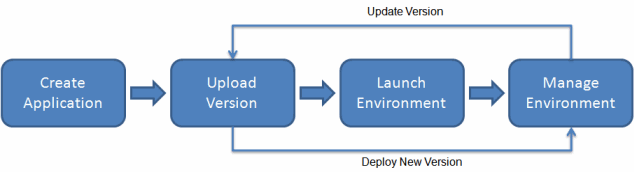
\includegraphics[width=0.5\textwidth]{figures/04_implementation/eb_flowchart}
    \caption{AWS Elastic Beanstalk Application Deployment}
\end{figure}

It is important that the EB application runs in the same availability zone of the VPC as JIRA, otherwise it wouldn't be reachable at all.

The database runs on managed Amazon RDS (Relational Database Service), which is fast, secure and scalable deployment of database engine. It manages backups, software patching, automatic failure detection, and recovery. The default database engine is MySQL.

\subsection{Spring Boot}

I first tried to use play2 framework for educational purposes, but I encountered too many obstacles deploying play2 application to AWS: 

\begin{itemize}
	\item It does not support WAR packaging.\footnote{There is an unofficial tool that packages the code in a WAR file, but it is not recommended for production environment. Being constrained by highly regulated market, something that already says that it is not production ready is an instant "No thanks".}
	\item It is not possible to run play2 packages (packaged by Activator tool) on Tomcat Server.
	\item It comes with its own Netty Server, which is really clumsy to set up in AWS environment.
\end{itemize}

All three combined resulted in inability to synchronize the play2 application on port 9000 and NGINX running on port 5000. Unfortunately Netty Server does not support compile-time port configuration and NGINX does not support running Activator to set up the port during run-time, so I had to drop the idea of using play2 as I was simply unable to deploy the application. After researching and discussing with my peers and coworkers I looked up Spring MVC and stumbled upon Spring Boot, also recommended by my classmate. I tried few sample apps and found out it supports WAR packaging, runs natively on Tomcat and comes with almost the same perks like play2. I was ready to give it a try.

"Spring Boot aims to make it easy to create Spring-powered, production-grade applications and services with minimum fuss. It takes an opinionated view of the Spring platform so that new and existing users can quickly get to the bits they need." \cite{spring-boot-blog}

Primary goals of Spring Boot are \cite{spring-boot-doc}:

\begin{itemize}
	\item Provide a radically faster and widely accessible getting started experience for all Spring development.
	\item Be opinionated out of the box, but get out of the way quickly as requirements start to diverge from the defaults.
	\item Provide a range of non-functional features that are common to large classes of projects (e.g. embedded servers, security, metrics, health checks, externalized configuration).
	\item Absolutely no code generation and no requirement for XML configuration.
\end{itemize}

\begin{figure}[!ht]
	\centering
	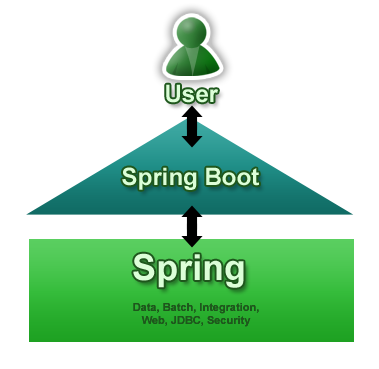
\includegraphics[width=0.4\textwidth]{figures/04_implementation/spring}
    \caption{Spring Boot architecture}
\end{figure}

The advantages seemed to be strong, development environment was convenient (native support in IntelliJ IDEA) and after some validation with Amazon support regarding AWS EB deployment in our VPC environment, I was confident this would be a good choice.

\subsection{Workflow}

...

\subsection{Technologies Used}

In order to make the development as comfortable as possible, I used various open-source frameworks/technologies to help me out with things that would otherwise take a lot of time

\subsubsection{H2 Database}

H2 is a Java SQL database that runs in-memory. It is great for fast prototyping and validating of design ideas before using production database (RDS). Due to the fact that the entire database is deleted after a server is restarted, it enabled me to quickly change the schema without the need to do tedious database wipes. 

Another great thing is that it only needs to be defined in pom.xml and all other linking is provided out-of-the-box:

\bigbreak

\begin{lstlisting}
<dependency>
    <groupId>com.h2database</groupId>
    <artifactId>h2</artifactId>
</dependency>
\end{lstlisting}

Important note: as it wires up all connections automatically, it is absolutely vital not to have {\bf any other} database engine loaded via Maven, otherwise it crashes on start-up of Tomcat.

\subsubsection{Flyway}

Flyway is an open-source database migration tool. It aims to be clean and simple rather than robust and too complex. It uses 6 main commands:

\begin{enumerate}
	\item Migrate - Migrates the schema to the latest version.
	\item Clean - Drops all objects in the configured schemas.
	\item Info - Prints the details and status information about all the migrations.
	\item Validate - Validates the applied migrations against the available ones.
	\item Baseline - Baselines an existing database, excluding all migrations upto and including baselineVersion.
	\item Repair - Repairs the metadata table.
\end{enumerate}

Since I didn't need to migrate the database, thanks to the flexibility of H2, I mainly used Flyway for cold start (empty database). I defined, what will be in the database after the server has started and Flyway filled it up for me.

\subsection{REST API}

// provides nice API

\subsection{Code Deployment}

The code is packaged by Maven and deployed as WAR file to AWS EB instance, running Tomcat 8 server. There is no need to configure anything with regards to basic networking - AWS EB is a back-to-back fully managed Platform as a Service (PaaS).

There are multiple things to consider when deploying to AWS EB, even though it seems "super-easy" in most instructional videos and ads:

\begin{enumerate}
	\item Contrary to programmer's logic, one has to first create an "Application" and under that custom "Environments". In other words, Application is the main context, and environments are servers running in the same context, by default having the permission to communicate between each other.
	\item In Environment setup, we can choose either a Web Server Environment or a Worker Environment. Web Server is the hub of any application and is used in both Semantic Data Manager and Tracking Engine. Workers are only used in Tracking Engine and will be explained later.
	\item Chosen configuration was obviously Tomcat and I also opted for automatic load balancing and scaling.
	\item Opting to automatically create an RDS instance along with the environment is a really bad design. Once an environment is terminated, so is the database instance which causes a serious data loss.
	\item In order to access the servers via SSH, it is necessary to define a EC2 Security Group and assign it accordingly. Otherwise, all outside access is prohibited.
	\item It is also crucial to wisely choose the instance type. I opted for m3.medium, because Java applciations by themselves are quite demanding and I didn't want to risk being on the edge when strange errors occur because of insufficient memory capacity.
	\item Permissions and roles are absolutely crucial when it is desired to connect the Environment with other AWS services, such as object storage (S3 = Simple Storage Service) or a messaging queue (SQS = Simple Queue Service).
\end{enumerate}

 The size of the instance is recommended for any application running JVM. The configuration is Intel Xeon E5-2670 v2 (Ivy Bridge), 4GB SSD storage and 3.75GB RAM. Any additional memory is handled via S3.

\subsection{User Interface}

The component Semantic Data Manager provides REST API to be consumed by any kind of client capable of HTTP requests. Because my specialization are mobile applications, I chose to implement a mobile application for iOS as an administrating user interface for this component.

\subsubsection{Application Flow}

SCREENSHOTS

\subsubsection{Technologies Used}

Moya, Alamofire

\section{Tracking Engine}

Tracking Engine is also deployed in AWS EB but uses Aurora as database engine. Aurora is ... and has ... configuration, allowing to have really high traffic and maintain its speed and robustness.

Because the tracking engine was developed after the Semantic Data Manager, I opted to use Java again. 

The code is deployed in the same fashion as the Semantic Data Manager.

\section{Tracked Device SDK}

TBD

\subsection{Technologies Used}

// Realm.IO
// Alamofire
// Moya
// GZIP